\documentclass[a4paper]{article}
\usepackage[utf8x]{inputenc}
\usepackage[german,ngerman]{babel}
\usepackage[a4paper,hmargin=2cm,vmargin=3cm]{geometry}
\usepackage[hyperindex=true]{hyperref}
\usepackage{tabularx}
\usepackage{graphics}
\usepackage{textcomp}

\setlength{\headheight}{27pt} % header with two lines
\setlength{\parindent}{0pt}
\setlength{\parskip}{4pt}

\title{Benutzerhandbuch}
\author{Christoph Peltz}

\begin{document}
\maketitle
\pagebreak
\tableofcontents
\pagebreak
	\section{Allgemeines zur Verwendung}


	\subsection{Aufbau des Protokolls}

	Das Protokoll ist Byte-orientiert und besteht aus Befehlen.
	Ein Befehl muss mindestens ein Byte lang sein, seine
	maximale Breite ist durch den Wert des Defines
	ORDER\_TYPE\_MAX\_LENGTH in der option.h gegeben (Standard: 15).
	Das erste Byte eines Befehls wird Kommando-Byte genannt und
	besteht aus zwei Teilen. Der erste Teil wird Befehlscode
	genannt und spezifiziert, welcher Befehl übermittelt wird.
	Der zweite Teil wird Option-Teil genannt. In ihm werden
	Optionen angegeben, die das Verhalten des Befehls modizifieren
	können. Manche Befehle benötigen keine Optionen, um zu
	funktionieren; andere hingegen schon. Die oberen (MSB) 4 Bit
	des Kommando-Bytes sind für Optionen reserviert, die unteren
	(LSB) 4 Bit für den Befehlscode. Die Bytes, die auf dem
	Kommando-Byte folgen sind Parameter. Es gibt eine Ausnahme
	diesr Regel: Der Befehl mit dem Befehlscode 0x00 kann mehrere
	Kommando-Bytes besitzen, doch dies muss explizit implementiert
	werden. Mehr hierzu findet man bei der Beschreibung des Befehls.
	\\
	Die Optionen, die bei den Befehlen angegeben sind, werden mit
	dem Befehlscode verodert, um das Kommando-Byte zu erhalten.
	Einige Optionen schließen sich gegenseitig aus, andere können
	kombiniert werden. Die genaue Verwendung der Optionen wird
	bei den einzelnen Befehlen genau erläutert.
	\\
	\begin{figure}[!ht]
		\centering
		\scalebox{0.3}{
			\fbox{
				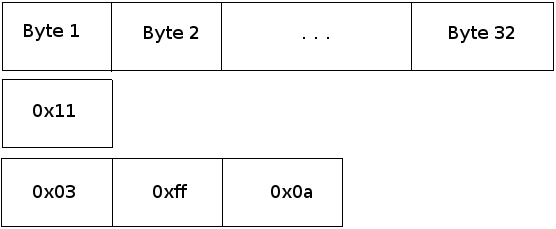
\includegraphics{Aufbau.png}
			}
		}
		\caption{Schematischer Aufbau eines Befehls und zweier Beispiele (mittleres ist ein Reset, unteres ein Fahrbefehl ohne
		Trigger mit den Geschwindigkeiten -128 und 10}
	\end{figure}
	
	\subsection{I2C-Bus}
	
	Die Adresse der Motorplatine am I2C-Bus ist 42. Die Motorplatine
	antwortet nicht auf die General-Call Adresse des I2C-Bus. Bei
	Befehlen, die eine Ausgabe zur Folge haben, muss die Praktikumsplatine
	von der Motorplatine lesen. Die Motorplatine wird von selbst nicht
	anfangen Daten über den I2C-Bus zu übermitteln. Außerdem muss der
	Motorplatine genügend Zeit gelassen werden, um die Antwort auf
	den übertragenen Befehl zu generieren und bereitzustellen (1 ms warten
	sollte genügen, eventuell ist es auch möglich nur 200 \textmu{}s zu
	warten).
	
	\subsection{UART-Port}
	
	Der UART-Port verwendet eine BAUD-Rate von 57600. Falls Debug-Ausgaben
	eingestellt sind, werden diese über den UART-Port ausgegeben. Das
	wir auch dann getan, wenn über UART Befehle empfangen werden. D.h.
	mit aktivierten Debug-Ausgaben kann von der Praktikumsplatine keine
	Werte ausgelesen werden (Antworten auf einen QUERY-Befehl zum Beispiel),
	da die Debug-Ausgaben wie normale Antworten aussehen.
	
	\subsection{Kompilieren und Überspielen auf die Motorplatine}
	
	Soll eine angepasste Version der Betriebssoftware für die Motorplatine
	kompiliert und auf diese überspielt werden, sind folgende Programme nötig:
	\begin{itemize}
		\item Der Quellcode (http://github.com/cpeltz/ba-arbeit)
		\item git Versions-Kontroll-System (http://en.wikipedia.org/wiki/Git\_(software);
		http://code.google.com/p/msysgit/)
		\item gcc-avr (http://winavr.sourceforge.net/)
	\end{itemize}
	Mit dem Ende der zugehörigen Bachelor-Arbeit wird, an passenden stellen, ein ''Tag''
	gesetzt. Nur ordentlich getagte commits sollten kompiliert werden, alle anderen
	können mit höherer Wahrscheinlichkeit Fehler enthalten. Zuerst sollte sowohl
	git als auch gcc-avr installiert werden und gcc-avr sollte in die PATH-Variable
	eingetragen werden. Danach kann das git-Repository an der oben genannten Adresse
	gecloned werden. Im Hauptverzeichniss des gecloneten Repositories gibt es eine
	''Makefile''. Ein einfacher Aufruf von ''make'' kompiliert das Programm. Der Aufruf
	"make program" kopiert das kompilierte Program über die serielle Schnittstelle,
	die mit einem speziellen AVR-Programmier-Board verbunden sein muss, auf die
	Motorplatine. Der Aufruf ''make clean'' entfernt alle kompilierten Dateien (ein
	''git clean -f'' säubert das gesamte Repository). Wie genau die Hardware anzuschließen
	ist kann in dem Benutzerhandbuch von Timo Klingeberg (http://www.ibr.cs.tu-bs.de/theses/broeke/SA\_Getriebemotorenansteuerung/) nachgelesen werden. Die Einstellungsschritte und
	das Programm AVR-Studio sind für die Entwicklung allerdings nicht nötig.

	\pagebreak


	\section{0x00 - Extended Instruction}

	\subsection{Kurzbeschreibung}

	Dieser Befehl ist für zukünftige Erweiterungen des Protokolls vorgesehen,
	falls mehr als 15 verschiedene Befehle benötigt werden. Wird dieser
	Befehlscode angetroffen, so werden nachfolgende Bytes als zusätzliche
	Kommando-Bytes gewertet und besonders behandelt. In der aktuellen
	Implementierung wird nur das erste Kommando-Byte eingelesen, danach gilt der
	Befehl als beendet. Bei der	Ausführung des Befehls wird nichts getan,
	nur der Befehlsstatus auf DONE gesetzt.

	\subsection{Referenz}

	Bisher werden Befehle mit diesem Code werden nach einem Byte abgebrochen
	und in die Queue gestellt. Es existiert noch keine Anwendung für diese
	Befehlsgattung.
	\\
	Die Funktionen, die die Besonderheiten dieses Befehls behandeln, befinden
	sich fast ausschließlich in der parse.c. Es ist die
	parser\_extended\_order\_complete()-Funktion, die eine 1 zurück geben muss,
	wenn der übergebene Befehl fertig empfangen wurde. Eventuell muss die
	parser\_check\_order()-Funktion für den Befehl angepasst werden. Außerdem
	muss die extended\_instruction()-Funktion in order\_functions.c implementiert
	werden.
	
	\pagebreak

	\section{0x01 - Control}

	\subsection{Kurzbeschreibung}
	
	Der Control-Befehl wird benutzt, um verschiedene Aspekte der Motorplatine
	zu kontrollieren. Dieser Befehl kann somit genutzt werden, um die
	Motorplatine zurückzusetzen, den aktuellen Befehl anzuhalten, oder
	um die Warteschlange zu steuern. Wichtig ist, dass dieser Befehl
	ein priorisierter Befehl ist. Das bedeutet: Er wird nicht an die
	Warteschlange angereiht, sondern wird umgehend nach Empfang in der
	nächsten Hauptschleifen-Iteration ausgeführt. Der bisher ausgeführte Befehl
	wird hierfür solange ausgesetzt, bis der priorisierte Befehl abgearbeitet
	wurde. Die bisher implementierten Optionen des Control-Befehls benötigen
	nur \textbf{eine} Hauptschleifen-Iteration. Es kann gleichzeitig nur
	ein priorisierer Befehl bearbeitet werden. Dies ist normalerweise kein
	Problem, da der kleinste Befehl über 500 \textmu{}s benötigt, um übertragen
	zu werden. Es dauert aber normalerweise ungefähr 300 \textmu{}s bis solch
	ein Befehl abgearbeitet wurde.


	\subsection{Referenz}

	\begin{tabularx}{\linewidth}{|l|l|X|}
		\hline
		\textbf{Option} & \textbf{Bitmaske} & \textbf{Beschreibung} \\
		\hline
		\hline
		Reset 			& 0x10 				& Zurücksetzen der Hardware \\
		\hline
		Stop Queue		& 0x20				& Der Aktuelle Befehl wird verworfen. Warteschlange wird angehalten, aber nicht verworfen. \\
		\hline
		Continue Queue	& 0x30				& Eine gestoppte Warteschlange wird fortgeführt. \\
		\hline
		Clear Queue		& 0x40				& Der Inhalt der Warteschlange wird gelöscht. \\
		\hline
		Stop Drive		& 0x50				& Aktueller Befehl wird angehalten, Fahrzeug geht zum aktiven Bremsen über (falls aktiviert). \\
		\hline
	\end{tabularx}

	Die Optionen schließen sich gegenseitig aus, d.h. es kann nur eine der
	Optionen gewählt werden. Der Control-Befehl ist 1 Byte lang, besteht also
	nur aus dem Kommando-Byte. Dieser Befehl gehört zu den priorisierten
	Befehlen. Er wird also nicht an die normale Warteschlange angereiht,
	sondern während der nächsten Hauptschleifen-Iteration ausgeführt.


	\subsection{Beispiele}
	
	\begin{verbatim}
		Reset: 0x01 OR 0x10 = 0x11
		Stop Drive: 0x01 OR 0x50 = 0x51
	\end{verbatim}
	
	\pagebreak

	\section{0x02 - Query}

	\subsection{Kurzbeschreibung}

	Der Query-Befehl dient zur Abfrage bestimmter Werte, die intern auf der
	Motorplatine benutzt werden. Der Befehl an sich weist die Motorplatine
	an die Daten auszugeben. Dies erfolgt bei Benutzung des UART-Ports so
	schnell wie möglich (nach ungefähr 300 \textmu{}s), bei der Benutzung
	des I2C-Busses sobald die Daten von der Praktikumsplatine abgefragt
	werden. Diese Abfrage sollte aber 300 \textmu{}s nach dem Empfangen
	des Befehls durchgeführt werden. Stehen die Daten noch nicht bereit,
	während sie angefordert werden, wird nicht zurückgegeben. Ein Aufruf
	von i2c\_send() oder order\_send() liefern daher 0 zurück.

	\subsection{Referenz}

	\begin{tabularx}{\linewidth}{|l|l|X|}
		\hline
		\textbf{Bitmaske} & \textbf{Beschreibung} & \textbf{Antwortlänge in Bytes} \\
		\hline
		\hline
		0x10 				& Geschwindigkeit des linken Rades & 1 \\
		\hline
		0x20				& Geschwindigkeit des rechten Rades & 1 \\
		\hline
		0x30				& Anzahl der Befehl in der Queue & 1 \\
		\hline
		0x40				& Aktueller Befehl & 2 - 16 (siehe Text) \\
		\hline
	\end{tabularx}

	Der Query-Befehl ist ein priorisierter Befehl und umgeht damit die
	Warteschlange. Das bedeutet: Er wird in der nächsten
	Hauptschleifen-Iteration nach seinem Empfang ausgeführt. Der Befehl
	hat eine konstante Länge von einem Byte, also nur das Kommando-Byte.
	Die oben aufgeführten Optionen schließen sich gegenseitig aus.
	Die Antworten dieses Befehls können eine variable Länge besitzen.
	So werden bei der Option 0x40 zwei Antworten generiert (nur für I2C-Bus
	wichtig: Es muss zweimal ein i2c\_recv() ausgeführt werden). Die erste
	gibt die Länge der zweiten Antwort an und die zweite erst enthält die
	angeforderten Daten. Die erste Antwort ist in diesem Fall aber immer
	ein Byte lang. Bei Befehlen mit konstanter Länge wird aber nur
	eine Antwort generiert.

	\subsection{Beispiele}

	\begin{verbatim}	
		Anzahl der Befehle: 0x02 OR 0x30 = 0x32
		Antwort (unter der Annahme, dass fünf
		Befehle in der Queue sind): 0x05
	\end{verbatim}
	\pagebreak


	\section{0x03 - Drive}

	\subsection{Kurzbeschreibung}
	
	Der Drive-Befehl ist der komplizierteste Befehl. Mit ihm kann das
	Fahrzeug bewegt werden. Hierbei kann die Geschwidigkeit aller Räder
	einzeln konfiguriert werden. Zustäzlich können Abbruch-Bedingungen
	für jedes Rad einzeln angegeben werden. Diese Abbruch-Bedingungen
	werden Trigger genannte. Es gibt momentan zwei verschiedene Trigger:
	Zeit-Trigger und Positions-Trigger. Zeit-Trigger halten das Rad an,
	nachdem sie eine bestimmte Zeit lang gelaufen sind. Positions-Trigger
	halten das Rad an, nachdem es eine bestimmte Anzahl an ''Ticks''
	gefahren ist (1 Tick = 1 Grad der Rades; d.h. 360 Ticks = 1
	Radumdrehung).
	\\
	Zusätzlich zu diesen Triggern besitzt der Drive-Befehl eine Option
	für einen speziellen Fahrmodus: Fahrt mit Differenzausgleich. Dieser
	Modus ist für die ''Geradeaus-Fahrt'' optimiert und ermöglicht es
	sehr genau geradeaus zu fahren. Zur Unterstützung dieses Modus
	gibt es eine weitere Option, die es erlaubt mit diesem Befehl den
	Startwert der Differenz zwischen den Rädern zu setzen.

	\subsection{Referenz}

	\begin{tabularx}{\linewidth}{|l|l|l|X|}
		\hline
		\textbf{Option} & \textbf{Bitmaske linkes Rad} & \textbf{Bitmaske rechtes Rad} & \textbf{Beschreibung} \\
		\hline
		\hline
		Kein Trigger	& 0x00						   & 0x00						   & Endlos-Fahrt \\
		\hline
		Zeit Trigger	& 0x10						   & 0x40						   & zeitlich begrenzte Fahrt\\
		\hline
		Positions Trigger & 0x20					   & 0x80						   & Fährt eine bestimmte Strecke \\
		\hline
	\end{tabularx}

	Aus dieser Liste muss je eine Bitmaske für das linke und das rechte
	Rad ausgewählt werden. Es sei denn, es wird eine der Bitmasken 0x30
	oder 0xc0 verwendet. Der Befehl erhält mindestens zwei Parameter:
	Die Geschwindigkeiten für das linke und rechte Rad. Beide
	Parameter haben eine Länge von einem Byte und sind vorzeichenbehaftet.
	Die Geschwindigkeit für das linke Rad wird vor der Geschwindigkeit
	des rechten Rades gesendet. Falls für eins oder mehr Räder Trigger
	ausgewählt wurden, werden deren Werte hinter den Geschwindigkeiten
	angegeben. Auch hier wird zuerst der Trigger-Wert für das linke Rad
	übermittelt, erst danach für das rechte Rad. Trigger-Werte sind
	2 Byte lang und vorzeichenlos.
	
	\begin{tabularx}{\linewidth}{|l|l|l|X|}
		\hline
		\textbf{Byte Anzahl} & \textbf{Option} & \textbf{Wertebereich} & \textbf{Beschreibung} \\
		\hline
		\hline
		1					 & - & -128 bis 127 & Geschwindigkeit des linken Rades \\
		\hline
		1					 & - & -128 bis 127 & Geschwindigkeit des rechten Rades\\
		\hline
		2					 & Zeit Trigger & 0 bis 65535 &  Zeit die das linke Rad fährt (in 100 ms)\\
		\hline
		2					 & Positions Trigger & 0 bis 65535 &  Anzahl der Ticks die das linke Rad fährt\\
		\hline
		2					 & Zeit Trigger & 0 bis 65535 &  Zeit die das rechte Rad fährt (in 100 ms)\\
		\hline
		2					 & Positions Trigger & 0 bis 65535 &  Anzahl der Ticks die das rechte Rad fährt\\
		\hline
	\end{tabularx}

	Der Befehl hat eine minimale Länge von 3 Byte (1 Kommando-Byte + je 1
	Byte für die Geschwindigkeiten). Maximal benötigt der Befehl 7 Byte
	(1 Kommando-Byte + je 1 Byte für die Geschwindigkeiten + je 2 Byte für
	die Trigger-Werte).
	\\
	\textbf{Die Bitmaske 0x30} spezifiziert die ''Fahrt mit Differenzausgleich''.
	Beide Räder werden hierbei so gesteuert, dass das Fahrzeug geradeaus fährt.
	Dadurch ist auch nur eine Geschwindigkeit notwendig, anstatt zwei. Es können
	immernoch Trigger verwendet werden. Die Bitmasken für die Trigger des rechten
	Rades werden für diesen Zweck benutzt. Beim benutzen der Trigger in desem
	Fahrmodus muss nur ein Triggerwert spezifiziert werden. Dieser wird dann für
	beide Räder benutzt; gleiches gilt für die Geschwindigkeit. Die minimale
	Länge verkürzt sich hierbei auf 2 Byte (1 Kommando-Byte + 1 Byte für die
	Geschwindigkeit) und die maximale auf 4 Byte (1 Kommando-Byte + 1 Byte für
	die Geschwindigkeit + 2 Byte für den Trigger-Wert).
	\\
	\textbf{Die Bitmaske 0xc0} wird verwendet, um die Anfangs-Differenz der Räder
	einzustellen. Der Befehl hat dann nur einen Parameter, der 2 Byte lang ist und
	vorzeichenbehaftet ist (-32768 bis 32767). Ein Wert gleich 0 setzt den Wert
	auf 0. Von 0 verschiedene Werte werden auf den aktuellen Differenzwert
	addiert. Die Länge des Befehls beträgt nun 3 Byte (1 Kommando-Byte + 2 Byte
	für den Differenzwert).

	\subsection{Beispiele}

	\begin{verbatim}
	Die Geschwindigkeit des linken Rades soll 100 betragen,
	die des rechten -50. Das linke Rad soll einen Zeit- und das
	rechte einen Positionstrigger verwenden. Die Zeit soll 500
	betragen, die Position 10000.
	Erstes Byte: 0x03 OR 0x10 OR 0x80 = 0x93
	Gesamte Befehl: 0x93 0x64 0xce 0x01 0xf4 0x27 0x10
	\end{verbatim}
	\pagebreak


	\section{0x04 - Advanced Drive}

	\subsection{Kurzbeschreibung}

	Der Advanced-Drive-Befehl bewegt wie der Drive-Befehl die Räder des
	Fahrzeugs. Die Besonderheit ist die Verknüpfung von Zeit- und
	Positions-Trigger. Es werden für jedes Rad beide Trigger benutzt, falls
	überhaupt Trigger verwendet werden. Es ist auch möglich, keine Trigger
	zu benutzen. Die Trigger werden, falls sie angegeben werden, miteinander
	logisch verknüpft. Dazu steht sowohl ein logisches UND als auch ein
	logisches ODER zur Verfügung. Damit ist es möglich, ein Rad mindestens
	2 Sekunden und 500 Ticks fahren zu lassen.
	
	\subsection{Referenz}

	\begin{tabularx}{\linewidth}{|l|l|l|X|}
		\hline
		\textbf{Option} & \textbf{Bitmaske linkes Rad} & \textbf{Bitmaske rechtes Rad} & \textbf{Beschreibung} \\
		\hline
		\hline
		Kein Trigger				& 0x00						   & 0x00						   & Endlos-Fahrt \\
		\hline
		Zeit ODER Position Trigger	& 0x10						   & 0x40						   & fährt bis einer der Trigger erreicht wurde\\
		\hline
		Zeit UND Positions Trigger  & 0x20						   & 0x80						   & fährt bis beide Trigger erreicht wurden \\
		\hline
	\end{tabularx}

	Die Bitmasken 0x30 und 0xc0 sind hier ungültig und dürfen nicht verwendet werden.
	Der ''Zeit ODER Position''-Trigger stoppt das Rad, wenn entweder der Zeit- oder der
	Positions-Trigger erreicht wurde. Beim ''Zeit UND Position''-Trigger wird das Rad
	gestoppt, wenn beide Trigger erreicht worden. Das bedeutet aber, dass für jedes Rad
	immer beide Trigger-Werte angegeben werden müssen. Dadurch, dass jetzt zwei Trigger
	gleichzeitig pro Rad angegeben werden, ist wichtig zu wissen, in welcher Reihenfolge
	diese übermittelt werden müssen. Dies zeigt die folgende Illustration:
	\begin{figure}[!ht]
		\centering
		\scalebox{1.0}{
				
\includegraphics{advanced_drive_instruction.png}
		}
		\caption{Ein Advanced-Drive-Befehl mit Zeit ODER Position Trigger für beide Räder (daher die 0x54)}
	\end{figure}
	Wenn kein Trigger verwendet wird, benötigt der Befehl 3 Byte (1 Kommando-Byte,
	je 1 Byte für die Geschwindigkeiten), wenn für beide Räder Trigger verwendet
	werden sind es im maximal Fall 11 Byte (1 Kommando-Byte, je 1 Byte für die
	Geschwindigkeiten, je 2*2 Byte für die Triggerwerte).

	\subsection{Beispiele}
	\pagebreak


	\section{0x05 - SetPID}

	\subsection{Kurzbeschreibung}

	Das PID-Modul ist die Haupt-Steuer-Einheit der Motorplatine.
	Es verwendet vier Parameter, die ihr Verhalten anpassen. Wie
	genau sich diese Parameter auswirken, ist in der Studienarbeit
	von Timo Klingeberg nachzulesen (http://www.ibr.cs.tu-bs.de/theses/
	broeke/SA\_Getriebemotorenansteuerung/download/studienarbeit.pdf).
	Das PID-Modul wird bereits mit Standard-Werten beim Start der
	Betriebssoftware programmiert. Daher ist es normalerweise nicht
	nötig diese anzupassen.


	\subsection{Referenz}

	\begin{tabularx}{\linewidth}{|l|l|l|X|}
		\hline
		\textbf{Byte Anzahl} & \textbf{Position} & \textbf{Wertebereich} & \textbf{Beschreibung} \\
		\hline
		\hline
		2					 & 1 & -32768 bis 32767 & Proportionaler Faktor\\
		\hline
		2					 & 2 & -32768 bis 32767 & Integraler Faktor\\
		\hline
		2					 & 3 & -32768 bis 32767 & Differentieller Faktor\\
		\hline
		2					 & 4 & -32768 bis 32767 & Maximale Fehlersummen Modifikator\\
		\hline
	\end{tabularx}

	Im Kommando-Byte muss angegeben werden, für welches Rad die Parameter gesetzt werden.

	\begin{tabularx}{\linewidth}{|l|X|}
		\hline
		\textbf{Option} & \textbf{Bitmaske} \\
		\hline
		\hline
		Linkes Rad	& 0x00 \\
		\hline
		Rechtes Rad	& 0x10 \\
		\hline
		Beide Räder & 0x20 \\
		\hline
	\end{tabularx}

	Die Länge des Befehls beträgt immer 9 Byte (1 Kommando-Byte + 4*2 Byte für die Variablen).

	\subsection{Beispiele}
	\pagebreak


	\section{0x06 - Option}

	\subsection{Kurzbeschreibung}

	Der Option-Befehl erlaubt es bestimmte Variablen der Motorplatine
	während der Laufzeit zu setzen. So kann das Aktive-Brems-System (ABS)
	mit diesem Befehl an die eigenen Bedürfnisse angepasst werden.

	\subsection{Referenz}

	Im Option-Teil wird die Variable spezifiziert, die gesetzt werden soll.
	Wichtig hierbei ist, dass das Kommando-Byte 0x06, also der Option-Teil
	gleich 0, für zukünftige Erweiterungen reserviert ist, damit mehr als
	16 Variablen mit diesem Befehl gesetzt werden können.

	\begin{tabularx}{\linewidth}{|l|l|l|X|}
		\hline
		\textbf{Bitmaske} & \textbf{Default} & \textbf{Wertebereich (Bytes)} & \textbf{Beschreibung} \\
		\hline
		\hline
		0x10 & 40 & 1 bis 127 (1) & Der Geschwindigkeitswert, der vom ABS benutzt wird. \\
		\hline
		0x20 & 1 & 0 oder 1 (1) & Switch zum aktivieren des ABS. Eine 1 bedeutet, dass das ABS aktiviert ist. \\
		\hline
		0x30 & 1 & 0 oder 1 (1) & Switch zum aktivieren des aktiven Bremsens, eines Rades, das bereits seinen Trigger erreicht hat. \\
		\hline
		0x40 & 1 & 0 oder 1 (1) & Switch zum aktivieren des aktiven Bremsens, wenn kein Befehl bearbeitet wird. \\
		\hline
	\end{tabularx}

	0x20 kann zum einfachen an- und ausschalten des ABS verwendet werden,
	die 0x30 und 0x40 Varianten sind für die Einschränkung des ABS, wenn es
	aktiviert ist, verantwortlich. 0x10 wird, wenn ein Wert außerhalb des Wertebereichs
	angegeben wird, den default-Wert benutzen. Momentan sind alle Option-Befehle 2 Byte lang.
	Der Status des ABS kann außerdem auf dem LCD abgelesen werden, falls es angeschlossen
	und aktiviert ist. ''AB:EIT'' ist die Angabe dafür, dass das aktive Bremsen (AB:) aktiviert
	(E; e wäre deaktiviert) ist. I bedeutet, dass das ABS für den Idle-Modus aktiviert wurde
	(i falls deaktiviert) und T gibt an, dass das ABS für das Erreichen eines Triggers
	aktiviert wurde (t falls deaktiviert).

	\subsection{Beispiele}
	\pagebreak

	
	\section{Verwendung der Befehls-Bibliothek}
	
	Die Befehls-Bibliothek ist optional und klein. Sie dient hauptsächlich dazu das Senden von Befehlen an
	die Motorplatine zu vereinfachen. Ohne die Bibliothek muss der Benutzer selber alle Felder eines Arrays
	korrekt setzen und sie selber senden. Die Bibliothek hingegen sellt eine große Menge an defines bereit,
	die das spätere lesen des Codes vereinfachen, sowie einige Funktionen, die das füllen der Parameter
	kurz und übersichtlich hält. Natürlich hat dies einen geringen Overhead zur Folge (mindestens wegen der
	Funktionsaufrufe).
	Um einen Befehl mit der Bibliothek zu erstellen und abzusenden sind folgende folgene Schritte durchzuführen:
	\begin{enumerate}
		\item Erstellen einer Variable vom Typ order\_t
		\item Initialisieren dieser Variable mit order\_init(order\_t)
		\item Einstellen des Befehlstypes mit order\_set\_type(order\_t, type) (Hierfür gibt es eine Menge an defines
			um diesen Aufruf kurz und informativ zu halten)
		\item Setzen, wenn nötig, der Parameter für den Befehl, mithilfe von order\_add\_params(order\_t, format, param1, ..., paramN)
		\item Senden des Befehls an die Platine mithilfe von order\_send(order\_t), order\_send\_and\_recv(order\_t) oder
			order\_send\_and\_recv\_co(order\_t).
	\end{enumerate}
	Wichtige Besonderheiten sind, dass der Typ order\_t, zwar größenteils identisch mit dem auf der Platine verwendete
	Typ ist, statt einer status-Variablen jetzt eine pos-Variable hat, die {\em nur intern verwendet} werden darf.
	Sie speichert die Schreibposition sowie die länge des Befehls. Das große data Array musste hier in dat umbenannt
	werden, da data ein reserviertes Wort unter Keil ist. Das erste Feld in dem dat Array speichert die Adresse der
	Platine und wird während order\_init(order\_t) gesetzt. Ab dem zweiten Feld des dat Array residieren hier nur die
	Befehlsdaten.
	Mit order\_set\_type(order\_t, type) wird der Typ des Befehls gesetzt, das bedeutet, das erste Byte des Befehls auch
	Befehlsbyte genannt. Für jeden validen Typ, das schließt auch alle Optionen mit ein, gibt es ein define, welches man
	hierfür verwenden kann.
	Die Funktion order\_add\_params(order\_t, format, param1, .., paramN) hat eine variable Anzahl an Parametern. Die
	Anzahl der Parameter und deren Typen wird durch den format-String festgelegt. Dieser besteht aus einer Kombination
	aus 1en und 2en. Die 1en bedeuten ein 1-Byte Parameter (int8\_t oder äquivalent) wobei die 2en ein 2-Byte
	Parameter bedeuten (int16\_t oder äquivalent). Sie werden in der Reihenfolge in der sie angegeben wurden auch erwartet
	und eingefügt. Beispiel: "1121" würde aussagen, dass zwei 1-Byte Parameter, dann ein 2-Byte Parameter, gefolgt von
	einem weiteren 1-Byte Parameter erwartet wird.
	Wenn der Befehl nun zur Zufriedenheit konstruiert wurde, kann er mit einem der drei send-Funktionen gesendet werden.
	Wichtig ist hier die Richtige auszuwählen. Dabei gilt, wird keine Antwort auf den Befehl erwartet (der Großteil der
	Befehle), dann wird order\_send(order\_t) benutzt. Die Funktion gibt die Anzahl der gesendeten Bytes zurück.
	Falls der Befehl eine Antwort provoziert (wie die query-Befehle), dann wird order\_send\_and\_recv(order\_t) benutzt.
	Dieser wird den Befehl senden und an die Stelle der Alten Befehlsdaten (also ab dem zweiten Feld) die Antwort einlesen.
	Außerdem gibt der Befehl die Anzahl der gelesenen Bytes zurück. (pos wird nicht korrekt gesetzt).
	Es gibt noch einen Befehl zum Senden und Empfangen, das ist der order\_send\_and\_recv\_co(order\_t). Dieser muss
	benutzt werden, wenn die Antwort der Platine eine variable Länge hat (so wie die Antwort auf den Query nach dem
	aktuellen Befehl (current order) von dem der Befehl auch seinen Namen ableitet. Auch dieser Befehl gibt die Anzahl
	der empfangenen Bytes zurück und speichert die empfangenen Daten ab dem zweiten Feld des dat-Arrays.

\end{document}
